\chapter{Lab 3}
\setcounter{TASignatures}{0}
\setcounter{AsideCounter}{0}

\section{Introduction}
    \vspace{0.1em}

    \textbf{In this lab you gain experience with:}
    \begin{enumerate}
        \item Arithmetic instructions
        \item Compare instructions
        \item Implementing counters without using a counter instruction
        \item Implementing modulo functionality without using a modulo instruction
    \end{enumerate}

\subsection{Lab Files}

Go to iLearn and download the PLC and HMI files for this lab to the PC. Then download the PLC project to the PLC and the HMI application to the HMI. 

\subsection{Acceptable Instructions}

You may have previous experience with PLCs and that is great! However, you are only allowed to use the instructions that we have covered thus far in the lab. So, if you have experience already, consider it a challenge to restrict yourself to only use the instructions that have been covered thus far in lecture to solve the problem!

You are \textbf{not} allowed to use the modulo instruction, the counter instructions, the compute instruction, or the compare instruction. And as always you are \textbf{not} allowed to use the oneshot instruction (or any of the other rising/falling edge instructions).

\subsection{Lab agreement}

The planning of a program is often a very social activity, however the actual writing of the code is always an individual pursuit. In this class it is very much the same. Students are welcome to verbally assist each other, but each person is required to write their own code and personally complete each lab. In this way each student will gain valuable experience with programming PLCs. 

\textbf{The undersigned person guarantees that any and all work demonstrated to the TA in regard to this lab is a result of their own work with no unauthorized help.}

\signatureSlot{Student (Print \& Sign)}


\section{Transmission Makers of America}

This section corresponds to the \verb|Lab3_1| object in the Lab3 PLC file.
\\ 
\\
Transmission Makers of America (not a real company) is a tier 1 supplier of transmissions to automakers in the US. Their transmissions contain multiple gear packs which engage and disengage to provide the varying speed to torque relationship that cars require. 

Transmissions are difficult to manufacture because they require the gears to be meshed with very little backlash, and they must not be under a large amount of squeeze. One way to achieve such a precise fit would be to build every component absolutely perfectly... But that is extremely cost prohibitive. So, instead of counting on perfection, Transmission Makers of America use precisely sized shims to adjust the overall mesh depth of the gears, brilliant! 

The problem they are having is that the formula to calculate the correct size shim is quite complicated. Often when their employees calculate the necessary shim thickness, there are small math errors that render the transmission unusable. They have contracted you to code the fomula into a PLC and display the correct shim thickness on the HMI. They have already created the HMI and it has been provided to you so all you have to do is move the correct shim thickness into the \verb|Shim_Thickness| attribute from \tableautorefname \ref{Table:Lab3_1Attributes}. 

\aside{Backlash is the term used to describe the amount of separation between two gears. So, given gear A and gear B which are meshed together, the backlash is the rotation gear A can have \textbf{without} causing gear B to rotate.}

\aside{Tier 1 auto suppliers are those which are under contract to supply automotive components directly to automakers like GM, Ford, Toyota, etc.}

In reality, Transmission Makers of America only has shims in a few sizes. So, they use the shim that is closest in size to the ideal which will be calculated in the PLC. 

\begin{align}
\label{equ:Shim}
\tiny
\frac{Gear\_Diameter \cdot \sin{(Backlash)} \cdot Pinion\_Gear\_Depth}{(Drag\_Torque \cdot 20) + 3} - 2.32
\end{align}


\subsection{How should the logic work?}

That's for you to figure out.

\subsection{The Inputs and Outputs}

To access any of the signals listed in \tableautorefname \ref{Table:Lab3_1Attributes}, use the syntax \verb|Lab3_1.| followed by the attribute name. 

\begin{table}[h]
\centering
\caption{Attributes available in Lab3\textunderscore 1}
\label{Table:Lab3_1Attributes}
\begin{tabular}{c c c}
\toprule
Attribute Name & Data Type & Type\\
\midrule
\verb|Backlash| & Real & Output \\
\verb|Pinion_Gear_Depth| &  Real & Output \\
\verb|Gear_Diameter| &  Real & Output \\
\verb|Drag_Torque| &  Real & Output \\
\midrule
\verb|Shim_Thickness| & Real & Input\\
\bottomrule
\end{tabular}
\end{table}

Write the appropriate logic in the associated rung in the PLC file.

\TASignatureSlot



\section{Challenge - Modulo}

This section corresponds to the \verb|Lab3_2| object in the Lab3 PLC file.
\\ 
\\
Another weekly challenge from the competition for which you signed up! Write the logic necessary to calculate the modulo of two operands while only using the truncate, add, subtract, multiply, and divide instructions. Store the modulo of \verb|OperandA| and \verb|OperandB| in \verb|Calculated_Modulo|.

You may choose to create a new tag to store a temporary result. This is acceptable. If you need help creating a new tag, refer to \figureautorefname \ref{fig:BooleanTagCreation1_l3}. If the data you intend to store in the tag is not a boolean value \textbf{make sure that the datatype of the tag you create matches the datatype which you intend to store}. For this problem you will probably need to create a tag with datatype "Dint" or possibly "Real".

\aside{The modulo operation is typically denoted by the \% symbol.}

\aside{The TRN (truncate) instruction can be found in the Allen Bradley instruction set manual that is available. The truncate instruction removes the decimal portion of a number and leaves it whole without any rounding. ie. $TRN(6.1)=6.0$ and $TRN(6.99)=6.0$}

\subsection{How should the logic work?}

The modulo command calculates the remainder from a division operation. So, given \verb|OperandA| and \verb|OperandB|, calculate the remainder from $OperandA/OperandB$. As an example, if \verb|OperandA| is 5 and \verb|OperandB| is 3, then $OperandA \% OperandB = 2$. As a second example, if \verb|OperandA| is 13 and \verb|OperandB| is 6, then $OperandA \% OperandB = 1$. As a third example, if \verb|OperandA| is 14 and \verb|OperandB| is 7, then $OperandA \% OperandB = 0$. As a final example, if \verb|OperandA| is 5 and \verb|OperandB| is 2, then $OperandA \% OperandB = 1$. 

\aside{One of the powerful uses of the modulo operation, is it's ability to identify positive and negative numbers. Notice in the final example, $5\%2 = 1$. If the remainder of any number is non-zero after being divided by 2, then that number is odd.}

\subsection{The Inputs and Outputs}

To access any of the signals listed in \tableautorefname \ref{Table:Lab3_2Attributes}, use the syntax \verb|Lab3_2.| followed by the attribute name. 

\begin{table}[h]
\centering
\caption{Attributes available in Lab3\textunderscore 2}
\label{Table:Lab3_2Attributes}
\begin{tabular}{c c c}
\toprule
Attribute Name & Data Type & Type\\
\midrule
\verb|OperandA| & Dint & Output \\
\verb|OperandB| & Dint & Output \\
\midrule
\verb|Calculated_Modulo| & Dint & Input\\
\bottomrule
\end{tabular}
\end{table}

Write the appropriate logic in the associated rung in the PLC file.

\TASignatureSlot


\section{7 Boxes and Counting}

This section corresponds to the \verb|Lab3_3| object in the Lab3 PLC file.
\\ 
\\

The online retailer (You signed an non-disclosure agreement so you can't speak their name) which contracted you to automate their box moving process has now become a repeat customer! They now want you to implement a counting system to count how many boxes have been transferred to trucks.

They intend to use the box transfer counter as a means of keeping each shift on track. Each shift is intended to transfer 7 heavy parcels. However, some shifts are not hitting their goal. So, by having a counter on the screen to keep track of their progress, the retailer hopes to increase productivity. 

They also want you to reset the count when the shift leader hits the reset button on the HMI. Moreover, they want you to send a signal to the HMI when the shift goal is met. 

\subsection{How should the logic work?}

Each time \verb|Start_Transfer| goes from false to true, they want you to increment the value stored in \verb|Current_Count| to keep track of the number of boxes that have been transferred. They also want you to reset the counter to 0 whenever the \verb|Reset_Counter| tag is true. Finally, if the value in \verb|Current_Count| is greater than or equal 7, you should turn on the \verb|Shift_Goal_Met| bit.


\subsection{The Inputs and Outputs}


To access any of the signals listed in \tableautorefname \ref{Table:Lab3_3Attributes}, use the syntax \verb|Lab3_3.| followed by the attribute name. 

\begin{table}[h]
\centering
\caption{Attributes available in Lab3\textunderscore 3}
\label{Table:Lab3_3Attributes}
\begin{tabular}{c c c}
\toprule
Attribute Name & Data Type & Type\\
\midrule
\verb|Start_Transfer| & Bool & Output \\
\verb|Reset_Counter| & Bool & Output \\
\midrule
\verb|Current_Count| & Dint & Input\\
\verb|Shift_Goal_Met| & Bool & Input\\
\bottomrule
\end{tabular}
\end{table}

Write the appropriate logic in the associated rung in the PLC file.

\TASignatureSlot

\newpage
\begin{samepage}
\begin{figure}[h]
\centering
\textbf{Open Parameters and Local Tags}\par \medskip
\frame{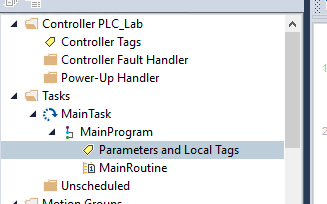
\includegraphics[width=3.2in]{BooleanTagCreation1}}
\caption{First step to creating a new boolean tag}
\label{fig:BooleanTagCreation1_l3}
\end{figure}



\begin{figure}[h]
\centering
\textbf{Create new Boolean Tag}\par \medskip
\frame{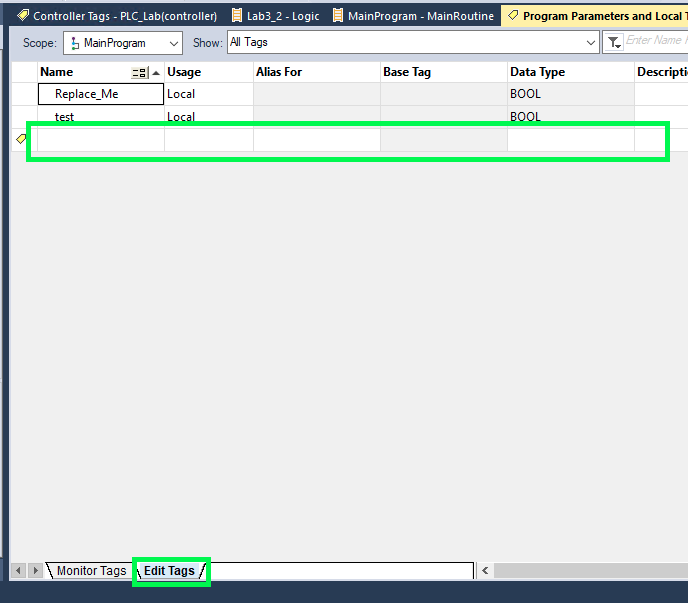
\includegraphics[width=3in]{EditTags}}
\caption{Second and Third step to creating a new boolean tag}
\label{fig:EditTags_l3}
\end{figure}

\section{How to create a boolean tag}
\label{Section:BooleanTag_l3}


To create another boolean tag to store the result of a boolean operation. Go to the left hand controller organizer menu. Under Main Program, double the item named Parameters and Local Tags. Refer to \figureautorefname \ref{fig:BooleanTagCreation1_l3}.



Next, in the window that appears insure that you are on the edit tab of the parameters and tags window. In \figureautorefname \ref{fig:EditTags_l3} you can see that the edit tab is in a green box for visibility at the bottom left. 

Finally, in the bottom entry in the list of tags enter the details for the tag that you are creating. The only two items that you should enter are the name and the datatype. The name must be a name that is not already taken and the datatype must be BOOL.
\end{samepage}